\documentclass[11pt,a4paper]{article}

\usepackage[margin=1in]{geometry}
\usepackage{graphicx}
\usepackage{booktabs}
\usepackage{amsmath}
\usepackage{hyperref}
\usepackage{caption}
\usepackage{subcaption}
\usepackage{float}
\usepackage{parskip}
\usepackage{titlesec}
\usepackage{xcolor}
\usepackage{tikz}
\usetikzlibrary{positioning,arrows.meta}

\hypersetup{colorlinks=true, linkcolor=blue, citecolor=blue, urlcolor=blue}

\title{\textbf{CNN vs.\ Vision Transformer for Image Classification on CIFAR-10}}
\author{Sneha Yadav}
\date{\today}

\begin{document}

\maketitle

% ─────────────────────────────────────────────────────────────────────────────
\section{Introduction}
% ─────────────────────────────────────────────────────────────────────────────

Convolutional Neural Networks (CNNs) have dominated computer vision for over a decade,
achieving state-of-the-art results on image classification benchmarks.
Recently, Vision Transformers (ViTs)~\cite{dosovitskiy2020vit} have emerged as a compelling
alternative, applying the self-attention mechanism—originally designed for natural language
processing—directly to sequences of image patches.

This report compares a CNN-based model (SmallResNet) and a Transformer-based model (ViT)
trained from scratch on CIFAR-10~\cite{krizhevsky2009cifar} under identical conditions.
Both models are sized to approximately 3\,M parameters so that any performance difference
is attributable to architecture rather than capacity.
The comparison covers three dimensions: \emph{performance} (accuracy),
\emph{efficiency} (parameters, FLOPs, training time, inference throughput), and
\emph{representation ability} (t-SNE visualisation and silhouette score).

% ─────────────────────────────────────────────────────────────────────────────
\section{Dataset}
% ─────────────────────────────────────────────────────────────────────────────

CIFAR-10 consists of 60{,}000 colour images ($32\times32$ pixels) evenly distributed
across 10 classes: \textit{airplane, automobile, bird, cat, deer, dog, frog, horse,
ship,} and \textit{truck}.
The standard split of 50{,}000 training images and 10{,}000 test images is used.

\textbf{Training augmentation.}
Random crop (padding of 4 pixels) and random horizontal flip are applied during training
to reduce overfitting.
Test images are only normalised using the per-channel mean
$\mu = (0.4914,\,0.4822,\,0.4465)$ and standard deviation
$\sigma = (0.2470,\,0.2435,\,0.2616)$.

% ─────────────────────────────────────────────────────────────────────────────
\section{Model Architectures}
% ─────────────────────────────────────────────────────────────────────────────

\subsection{SmallResNet (CNN)}

The CNN is a custom residual network inspired by ResNet~\cite{he2016resnet}.
It consists of a stem convolution followed by three stages of residual blocks,
as summarised in Table~\ref{tab:cnn_arch}.

\begin{table}[H]
\centering
\caption{SmallResNet architecture for a $3\times32\times32$ input.}
\label{tab:cnn_arch}
\begin{tabular}{llcc}
\toprule
\textbf{Layer / Stage} & \textbf{Operation} & \textbf{Output shape} & \textbf{Channels} \\
\midrule
Input  & ---                              & $3\times32\times32$   & 3   \\
Stem   & Conv $3\times3$, BN, ReLU        & $64\times32\times32$  & 64  \\
Stage 1 & $2\times$ ResidualBlock(64)     & $64\times32\times32$  & 64  \\
Stage 2 & $2\times$ ResidualBlock(128, s=2)& $128\times16\times16$& 128 \\
Stage 3 & $2\times$ ResidualBlock(256, s=2)& $256\times8\times8$  & 256 \\
Pooling & Global average pooling          & $256$                 & --- \\
Head   & Linear($256 \to 10$)             & $10$                  & --- \\
\bottomrule
\end{tabular}
\end{table}

Each \textbf{ResidualBlock} follows the standard post-activation residual design of He et al.~\cite{he2016resnet}:
\[
\mathbf{y} = \text{ReLU}\bigl(\text{BN}(\text{Conv}_2(\text{ReLU}(\text{BN}(\text{Conv}_1(\mathbf{x}))))) + \mathbf{x}\bigr)
\]
A $1\times1$ projection shortcut is used when the spatial size or channel count changes.
Total trainable parameters: \textbf{2.78\,M}.

\begin{figure}[H]
\centering
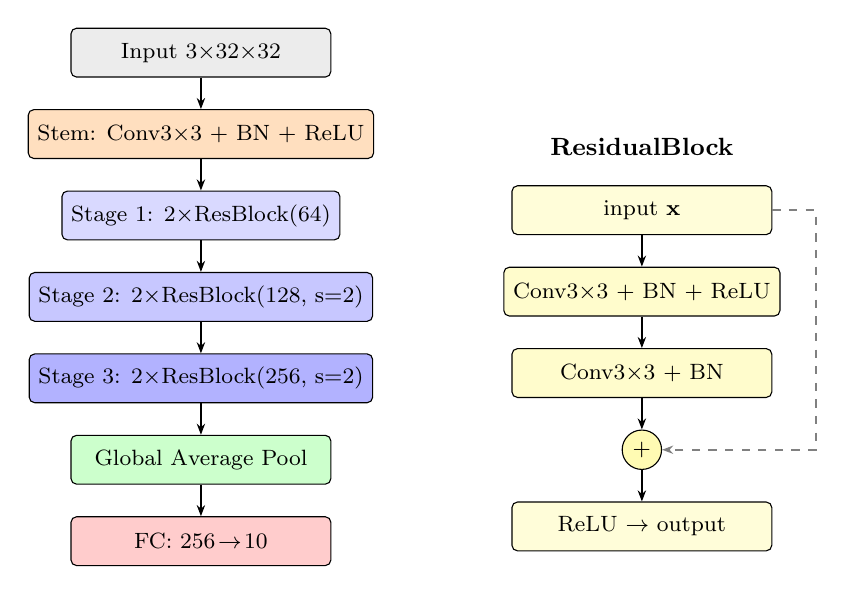
\begin{tikzpicture}[
  box/.style={draw, rounded corners=2pt, minimum width=3.3cm,
              minimum height=0.62cm, text centered, font=\footnotesize},
  circ/.style={draw, circle, minimum size=0.5cm, font=\footnotesize, inner sep=0pt},
  arr/.style={-{Stealth[length=4pt]}, thick},
  node distance=0.4cm
]
%% Left: main architecture flow
\node[box, fill=gray!15]                  (inp)  {Input $3{\times}32{\times}32$};
\node[box, fill=orange!25, below=of inp]  (stem) {Stem: Conv$3{\times}3$ + BN + ReLU};
\node[box, fill=blue!15,   below=of stem] (s1)   {Stage 1: $2{\times}$ResBlock(64)};
\node[box, fill=blue!22,   below=of s1]   (s2)   {Stage 2: $2{\times}$ResBlock(128, s=2)};
\node[box, fill=blue!30,   below=of s2]   (s3)   {Stage 3: $2{\times}$ResBlock(256, s=2)};
\node[box, fill=green!20,  below=of s3]   (gap)  {Global Average Pool};
\node[box, fill=red!20,    below=of gap]  (fc)   {FC: $256\!\to\!10$};
\foreach \a/\b in {inp/stem,stem/s1,s1/s2,s2/s3,s3/gap,gap/fc}
  \draw[arr] (\a) -- (\b);
%% Right: ResidualBlock detail
\begin{scope}[xshift=5.6cm, yshift=-1.2cm]
  \node[font=\small\bfseries]                        (rlabel) {ResidualBlock};
  \node[box, fill=yellow!15, below=0.25cm of rlabel] (rx)     {input $\mathbf{x}$};
  \node[box, fill=yellow!20, below=0.4cm of rx]      (rc1)    {Conv$3{\times}3$ + BN + ReLU};
  \node[box, fill=yellow!20, below=0.4cm of rc1]     (rc2)    {Conv$3{\times}3$ + BN};
  \node[circ, fill=yellow!30, below=0.4cm of rc2]    (ra)     {$+$};
  \node[box, fill=yellow!15, below=0.4cm of ra]      (rout)   {ReLU $\to$ output};
  \foreach \a/\b in {rx/rc1,rc1/rc2,rc2/ra,ra/rout}
    \draw[arr] (\a) -- (\b);
  \draw[arr, dashed, gray] (rx.east) -- ++(0.55,0) |- (ra.east);
\end{scope}
\end{tikzpicture}
\caption{SmallResNet architecture. \textbf{Left}: layer-by-layer flow from input to output.
         \textbf{Right}: internals of one ResidualBlock; the dashed line is the skip connection.}
\label{fig:cnn_diag}
\end{figure}

\subsection{Vision Transformer (ViT)}

The ViT follows the architecture introduced by Dosovitskiy et al.~\cite{dosovitskiy2020vit},
adapted for $32\times32$ images.
The image is divided into non-overlapping $4\times4$ patches, yielding 64 tokens.
A learnable \texttt{[CLS]} token is prepended, and learnable positional embeddings are
added before the transformer blocks (Table~\ref{tab:vit_arch}).

\begin{table}[H]
\centering
\caption{ViT architecture for a $3\times32\times32$ input.}
\label{tab:vit_arch}
\begin{tabular}{llcc}
\toprule
\textbf{Component} & \textbf{Operation} & \textbf{Output shape} & \textbf{Dim} \\
\midrule
Input            & ---                                   & $3\times32\times32$ & --- \\
Patch embedding  & Conv $4\times4$, stride 4             & $64\times256$       & 256 \\
CLS token        & Prepend learnable token               & $65\times256$       & 256 \\
Pos.\ embedding  & Add learnable position vectors        & $65\times256$       & 256 \\
Transformer      & $6\times$ TransformerBlock (8 heads, MLP dim 512) & $65\times256$ & 256 \\
LayerNorm        & Normalise all tokens, keep \texttt{[CLS]} & $256$               & --- \\
Head             & Linear($256\to10$)                    & $10$                & --- \\
\bottomrule
\end{tabular}
\end{table}

Each \textbf{TransformerBlock} uses pre-norm multi-head self-attention with dropout (0.1)
and a two-layer MLP with GELU activation:
\[
\mathbf{z} = \mathbf{x} + \text{MHSA}(\text{LN}(\mathbf{x})), \qquad
\mathbf{y} = \mathbf{z} + \text{MLP}(\text{LN}(\mathbf{z}))
\]
Total trainable parameters: \textbf{3.20\,M}.

\begin{figure}[H]
\centering
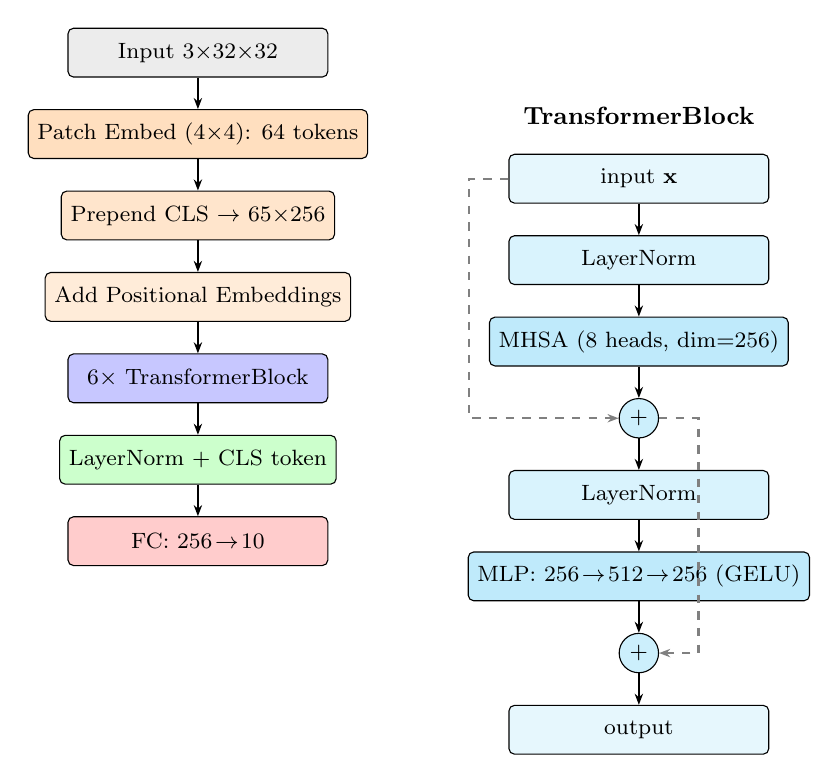
\begin{tikzpicture}[
  box/.style={draw, rounded corners=2pt, minimum width=3.3cm,
              minimum height=0.62cm, text centered, font=\footnotesize},
  circ/.style={draw, circle, minimum size=0.5cm, font=\footnotesize, inner sep=0pt},
  arr/.style={-{Stealth[length=4pt]}, thick},
  node distance=0.4cm
]
%% Left: main ViT flow
\node[box, fill=gray!15]                 (inp)  {Input $3{\times}32{\times}32$};
\node[box, fill=orange!25, below=of inp] (pe)   {Patch Embed ($4{\times}4$): 64 tokens};
\node[box, fill=orange!20, below=of pe]  (cls)  {Prepend CLS $\to$ $65{\times}256$};
\node[box, fill=orange!15, below=of cls] (pos)  {Add Positional Embeddings};
\node[box, fill=blue!22,   below=of pos] (tb)   {$6{\times}$ TransformerBlock};
\node[box, fill=green!20,  below=of tb]  (ln)   {LayerNorm + CLS token};
\node[box, fill=red!20,    below=of ln]  (fc)   {FC: $256\!\to\!10$};
\foreach \a/\b in {inp/pe,pe/cls,cls/pos,pos/tb,tb/ln,ln/fc}
  \draw[arr] (\a) -- (\b);
%% Right: TransformerBlock detail
\begin{scope}[xshift=5.6cm, yshift=-0.8cm]
  \node[font=\small\bfseries]                         (tlabel) {TransformerBlock};
  \node[box, fill=cyan!10,  below=0.25cm of tlabel]  (tx)     {input $\mathbf{x}$};
  \node[box, fill=cyan!15,  below=0.4cm of tx]       (tln1)   {LayerNorm};
  \node[box, fill=cyan!25,  below=0.4cm of tln1]     (tmha)   {MHSA (8 heads, dim=256)};
  \node[circ, fill=cyan!20, below=0.4cm of tmha]     (ta1)    {$+$};
  \node[box, fill=cyan!15,  below=0.4cm of ta1]      (tln2)   {LayerNorm};
  \node[box, fill=cyan!25,  below=0.4cm of tln2]     (tmlp)   {MLP: $256\!\to\!512\!\to\!256$ (GELU)};
  \node[circ, fill=cyan!20, below=0.4cm of tmlp]     (ta2)    {$+$};
  \node[box, fill=cyan!10,  below=0.4cm of ta2]      (tout)   {output};
  \foreach \a/\b in {tx/tln1,tln1/tmha,tmha/ta1,ta1/tln2,tln2/tmlp,tmlp/ta2,ta2/tout}
    \draw[arr] (\a) -- (\b);
  \draw[arr, dashed, gray] (tx.west)   -- ++(-0.5,0) |- (ta1.west);
  \draw[arr, dashed, gray] (ta1.east)  -- ++(0.5,0)  |- (ta2.east);
\end{scope}
\end{tikzpicture}
\caption{ViT architecture. \textbf{Left}: pipeline from input to output.
         \textbf{Right}: internals of one TransformerBlock; dashed lines are residual connections.}
\label{fig:vit_diag}
\end{figure}

% ─────────────────────────────────────────────────────────────────────────────
\section{Training Setup}
% ─────────────────────────────────────────────────────────────────────────────

Both models are trained with the \emph{identical} recipe to ensure a fair comparison:

\begin{itemize}
  \item \textbf{Optimiser:} AdamW, weight decay $5\times10^{-2}$
  \item \textbf{Learning rate:} $10^{-3}$, decayed to 0 via cosine annealing
  \item \textbf{Loss:} Cross-entropy with label smoothing $\varepsilon = 0.1$
  \item \textbf{Batch size:} 128
  \item \textbf{Epochs:} 30
  \item \textbf{Hardware:} NVIDIA GPU (CUDA)
  \item \textbf{Seed:} 0 (fixed random seed; GPU results may still vary slightly between runs)
\end{itemize}

% ─────────────────────────────────────────────────────────────────────────────
\section{Results}
% ─────────────────────────────────────────────────────────────────────────────

\subsection{Summary Table}

Table~\ref{tab:summary} reports the key metrics for both models after 30 epochs.

\begin{table}[H]
\centering
\caption{Performance and efficiency comparison on CIFAR-10. Time per epoch covers training only;
throughput is measured on the GPU with batches of 256.}
\label{tab:summary}
\begin{tabular}{lcc}
\toprule
\textbf{Metric} & \textbf{CNN (ResNet)} & \textbf{ViT} \\
\midrule
Parameters (M)              & 2.78  & 3.20  \\
FLOPs per image (M)         & 842   & 436   \\
Best test accuracy (\%)     & 92.62 & 73.76 \\
Final test accuracy (\%)    & 92.62 & 73.76 \\
Final train accuracy (\%)   & 99.57 & 77.31 \\
Total training time (min)   & 24.9  & 21.5  \\
Time per epoch (s)          & 49.8  & 42.9  \\
Inference throughput (img/s)& 2{,}351 & 4{,}241 \\
Peak GPU memory (MB)        & 749     & 815     \\
\bottomrule
\end{tabular}
\end{table}

\subsection{Learning Curves}

\begin{figure}[H]
  \centering
  \includegraphics[width=\textwidth]{curves.png}
  \caption{Training loss, test loss, and test accuracy over 30 epochs.}
  \label{fig:curves}
\end{figure}

Figure~\ref{fig:curves} shows that the CNN converges much faster and more steeply.
By epoch 10 it already reaches 87.2\% test accuracy, while the ViT is still at 63.0\%.
The CNN reaches 99.6\% training accuracy by epoch 30, indicating it has fully fit
the training data, whereas the ViT only reaches 77.3\%—suggesting it is underfitting
rather than overfitting.
(Training accuracy is measured during each epoch, with augmentation and dropout active.)

\subsection{Per-class Accuracy}

\begin{figure}[H]
  \centering
  \includegraphics[width=\textwidth]{per_class.png}
  \caption{Per-class test accuracy for CNN and ViT.}
  \label{fig:perclass}
\end{figure}

As shown in Figure~\ref{fig:perclass}, the CNN outperforms the ViT on every single class.
The hardest class for both models is \textit{cat}: the CNN achieves 82.1\% and the ViT
only 52.3\%.
The CNN performs best on \textit{automobile} (96.9\%) and \textit{ship} (96.3\%);
the ViT on \textit{ship} (85.9\%) and \textit{frog} (84.3\%).
These classes have globally distinctive shapes that are easier to separate even with weaker local features.

\subsection{Confusion Matrices}

\begin{figure}[H]
  \centering
  \includegraphics[width=\textwidth]{confusion.png}
  \caption{Normalised confusion matrices for CNN (left) and ViT (right).}
  \label{fig:confusion}
\end{figure}

The CNN's confusion matrix (Figure~\ref{fig:confusion}, left) is nearly diagonal,
indicating clean predictions across all classes.
The ViT (right) shows notable confusion between visually similar classes:
21\% of \textit{cat} images are misclassified as \textit{dog}, and 14\% of \textit{dog}
images are misclassified as \textit{cat}.
This reflects the ViT's weaker local texture discrimination at low resolution.

\subsection{Representation Ability: t-SNE}

\begin{figure}[H]
  \centering
  \includegraphics[width=\textwidth]{tsne.png}
  \caption{2-D t-SNE projection of 256-dimensional feature vectors from 2{,}000 test images.}
  \label{fig:tsne}
\end{figure}

Figure~\ref{fig:tsne} visualises the internal representations learned by each model.
The CNN forms tight, well-separated clusters with a \textbf{silhouette score of 0.421}.
The ViT's clusters heavily overlap, yielding a \textbf{silhouette score of only 0.130}.
This confirms that the CNN has learned more discriminative feature representations
from the limited CIFAR-10 training data.

% ─────────────────────────────────────────────────────────────────────────────
\section{Discussion}
% ─────────────────────────────────────────────────────────────────────────────

\subsection{Performance}

The CNN achieves \textbf{92.6\%} test accuracy versus \textbf{73.8\%} for the ViT—an
18.9 percentage point gap.
This gap is consistent with the broader literature: ViTs trained from scratch on small
datasets consistently underperform CNNs.
Dosovitskiy et al.\ themselves noted that ViTs require large-scale pretraining
(e.g., ImageNet-21k with 14\,M images, or JFT-300M with 300\,M images) to match or
surpass CNNs.
CIFAR-10 has only 50{,}000 training images—two to four orders of magnitude fewer.

A key indicator of the ViT's struggle is its \textbf{training accuracy of only 77.3\%},
compared to 99.6\% for the CNN. The CNN fits the training data almost perfectly and shows
a moderate train--test gap of 6.9 points (mild overfitting). The ViT's gap is only 3.6 points,
but both its training and test accuracy are low: the ViT is \emph{underfitting}, meaning it
has not yet learned the training data, let alone generalised from it.
Two factors contribute to this underfitting.
First, 30 epochs is a short training budget for a model that must learn all spatial
structure from scratch through attention, rather than relying on convolutional
inductive biases.
Second, no learning-rate warm-up was used. Transformers usually train more stably when
the learning rate is increased gradually over the first few epochs, because large early
updates can destabilise attention and LayerNorm.
Given more epochs or a warm-up schedule, the ViT's accuracy would likely improve,
though it would still lag behind the CNN on a dataset this small.

\subsection{Efficiency}

Interestingly, the ViT uses \textbf{fewer FLOPs} (436\,M vs.\ 842\,M per image) and
achieves \textbf{higher inference throughput} (4{,}241 vs.\ 2{,}351 images/s), despite
having more parameters.
This is because the ViT reduces the image to 65 tokens in its very first layer, whereas
the CNN's first stage runs $3\times3$ convolutions over the full $32\times32$ spatial grid
at multiple channel depths.
Peak training memory is similar, slightly higher for the ViT (815\,MB vs.\ 749\,MB),
because each block stores attention maps and MLP activations for all 65 tokens.
Training time per epoch is also slightly lower for the ViT (42.9\,s vs.\ 49.8\,s).
In a regime where only inference speed and FLOPs matter—not accuracy—the ViT would be
the more efficient choice.

\subsection{Representation Ability}

The silhouette score gap, computed on the 256-dimensional features (0.421 CNN vs.\ 0.130 ViT), is the clearest indication
of why the accuracy gap exists.
CNNs have two strong inductive biases built into their architecture:
(1) \emph{locality}—convolution kernels operate on spatially adjacent pixels, capturing
local textures and edges; and
(2) \emph{translation equivariance}—the same feature detector is applied at every
spatial location.
Both biases align naturally with the structure of natural images.

ViTs have only weak versions of these biases (locality exists only within each
$4\times4$ patch).
Self-attention has no built-in preference for nearby patches, so the model must
learn spatial relationships from data alone.
With only 50{,}000 images and 30 epochs of training, the ViT has not yet discovered
these relationships, resulting in poorly separated feature clusters.

\subsection{The cat/dog Problem}

Both models struggle most with \textit{cat} and \textit{dog}, but the ViT's confusion
is far more severe (21\% of cats predicted as dogs).
These two classes share similar local textures (fur, ears, snout) that require
fine-grained local feature extraction—precisely the strength of convolutional layers.
Transformers, without explicit local feature detectors, struggle to distinguish them
at $32\times32$ resolution.

% ─────────────────────────────────────────────────────────────────────────────
\section{Interactive Demo}
% ─────────────────────────────────────────────────────────────────────────────

The trained models are deployed in a Streamlit web app (\texttt{app.py}) that allows
uploading any image or picking a random CIFAR-10 test image to compare both models
side by side.

\begin{figure}[H]
  \centering
  % TODO: upload screenshot to Overleaf and replace "ui_input.png" with the actual filename
  \includegraphics[width=0.85\textwidth]{ui_input.png}
  \caption{App input view: a random CIFAR-10 test image (a bird) is selected.
           The left panel shows the original image; the right panel shows the
           32$\times$32 pixel version actually fed to both models.
           The true label is displayed as a blue info banner.}
  \label{fig:ui_input}
\end{figure}

\begin{figure}[H]
  \centering
  % TODO: upload screenshot to Overleaf and replace "ui_output.png" with the actual filename
  \includegraphics[width=0.85\textwidth]{ui_output.png}
  \caption{App output view for the same bird image. Both models correctly predict
           \textit{bird}—CNN at 88.3\% confidence and ViT at 91.3\%—and the green
           banner confirms agreement. This is one of the easier classes for both models;
           on harder classes such as \textit{cat}, the models frequently disagree.}
  \label{fig:ui_output}
\end{figure}

% ─────────────────────────────────────────────────────────────────────────────
\section{Conclusion}
% ─────────────────────────────────────────────────────────────────────────────

This experiment confirms that for image classification on a small dataset like CIFAR-10,
a CNN-based model (SmallResNet, 92.6\%) significantly outperforms a comparably-sized
Vision Transformer (ViT, 73.8\%) trained from scratch under identical conditions.

The CNN's advantage stems from its architectural inductive biases—locality and
translation equivariance—which align with the structure of natural images and allow
it to learn discriminative features from limited data.
The ViT, despite having fewer FLOPs and higher throughput, underfits: with no convolutional
priors, it needs longer training and a warm-up schedule, and ultimately far more data, to match the CNN.

These results are not an indictment of Transformers as a vision architecture.
When pretrained on hundreds of millions of images, ViTs match or surpass CNNs.
However, in data-limited settings, the inductive biases of CNNs remain a decisive
advantage.

% ─────────────────────────────────────────────────────────────────────────────
\begin{thebibliography}{9}

\bibitem{dosovitskiy2020vit}
A.~Dosovitskiy et al.,
``An Image is Worth 16x16 Words: Transformers for Image Recognition at Scale,''
\textit{ICLR}, 2021.

\bibitem{he2016resnet}
K.~He, X.~Zhang, S.~Ren, and J.~Sun,
``Deep Residual Learning for Image Recognition,''
\textit{CVPR}, 2016.

\bibitem{krizhevsky2009cifar}
A.~Krizhevsky,
``Learning Multiple Layers of Features from Tiny Images,''
Technical Report, University of Toronto, 2009.

\end{thebibliography}

\end{document}